\chapter{Sistema di raccomandazione}
\label{cap:sistema-raccomandazione}

\intro{In questo capitolo, vengono descritte le teorie e le tecniche utilizzate per il sistema di raccomandazione, con particolare attenzione allo studio dei sistemi reali, delle tecniche di raccomandazione, di combinazione e di valutazione dei risultati. Viene inoltre dato un accenno ai temi della Serendipità e dell'Explainability, oggetto di studio del progetto sebbene non implementati allo stato dell'arte.}

\section{Requisiti per il dataset}

Perchè sia possibile implementare un sistema di raccomandazione per e-commerce, è necessario che il dataset contenga le informazioni necessarie per poter effettuare le raccomandazioni. In particolare, è necessario che il dataset contenga:
\begin{itemize}
    \item \textbf{ID Cliente}: un identificativo univoco per ogni cliente, che permette di distinguere tra i diversi clienti del servizio di e-commerce;
    \item \textbf{SKU Prodotto}: un identificativo univoco per ogni prodotto, che permette di distinguere tra i diversi prodotti del servizio di e-commerce;
    \item \textbf{Nome Cliente}: il nome del cliente, che permette di identificare quest'ultimo in modo più intuitivo; a differenza dell'ID Cliente, il nome non deve necessariamente essere univoco, cioè può essere condiviso da più clienti;
    \item \textbf{Nome Prodotto}: il nome del prodotto, che permette di identificare quest'ultimo in modo più intuitivo; a differenza dell'SKU Prodotto, il nome non deve necessariamente essere univoco, cioè può essere condiviso da più prodotti.
\end{itemize}

Queste informazioni vengono dunque richieste in input come colonne del file \gls{csv} che contiene il dataset. L'\gls{llm} ha il compito di riconoscere quali colonne del file CSV ne sono rappresentanti, dopodichè i nomi corrispondenti vengono standardizzati rispettivamente in: \texttt{"Customer ID"}, \texttt{"Product SKU"}, \texttt{"Customer Name"} e \texttt{"Product Name"}. Queste colonne vengono dunque poi utilizzate per implementare le tecniche di raccomandazione, che si basano sull'analisi delle interazioni tra i clienti e i prodotti e sulla loro similarità.


\section{Collaborative filtering}

Il primo sistema che è stato esplorato è il \textbf{Collaborative Filtering}\footcite{site:collaborative-filtering}. Questo approccio si basa sull'idea che le raccomandazioni possono essere fatte in base alle preferenze di altri utenti simili. In altre parole, se due utenti hanno gusti simili, le raccomandazioni per uno di essi possono essere utili anche per l'altro. Il Collaborative Filtering può essere implementato in due modi principali: \textbf{user-based} e \textbf{item-based}. Nel primo caso, si analizzano le preferenze degli utenti per raccomandare prodotti che altri utenti simili hanno apprezzato. Nel secondo caso, si analizzano le caratteristiche dei prodotti per raccomandare articoli simili a quelli già apprezzati dall'utente. Dopo aver svolto alcune sperimentazioni pratiche con entrambi i metodi, si è notato che i dataset disponibili contenevano spesso troppi clienti occasionali che non avevano interagito con un numero sufficiente di prodotti per poter fare raccomandazioni significative, e questo ha messo in crisi il sistema \textbf{user-based}. Inoltre, si è pensato che, in generale, per un file delle vendite di un e-commerce, sia comune la presenza di utenti occasionali. Per questo motivo, si è deciso di implementare il sistema \textbf{item-based}, che si basa sulla similarità tra i prodotti piuttosto che sulle preferenze degli utenti. Infatti, siccome i comuni dataset di vendita sono ben forniti di informazioni sui propri prodotti, questo approccio consente di fare raccomandazioni più robuste e significative.

Nel contesto del Collaborative Filtering item-based, il processo di generazione delle raccomandazioni può essere formalizzato attraverso una serie di passaggi matematici ben definiti.

\subsection{Costruzione della matrice utente-prodotto}

Il primo passo consiste nella costruzione di una matrice di interazioni $\mathbf{R} \in \mathbb{R}^{m \times n}$, dove $m$ rappresenta il numero di utenti e $n$ il numero di prodotti. Ogni elemento $r_{ij}$ della matrice rappresenta il numero di interazioni (acquisti, visualizzazioni, etc.) dell'utente $i$ con il prodotto $j$:

\begin{equation}
\mathbf{R} = \begin{bmatrix}
r_{11} & r_{12} & \cdots & r_{1n} \\
r_{21} & r_{22} & \cdots & r_{2n} \\
\vdots & \vdots & \ddots & \vdots \\
r_{m1} & r_{m2} & \cdots & r_{mn}
\end{bmatrix}
\end{equation}

dove $r_{ij} = \sum_{k} \delta(u_k = i \land p_k = j)$ e $\delta$ è la funzione indicatrice che vale 1 se l'utente $i$ ha interagito con il prodotto $j$, 0 altrimenti.

\subsection{Calcolo della matrice di similarità prodotto-prodotto}

La matrice di similarità $\mathbf{S} \in \mathbb{R}^{n \times n}$ viene calcolata utilizzando la similarità coseno tra i vettori prodotto. Ogni prodotto $j$ è rappresentato dal vettore colonna $\mathbf{r}_j = [r_{1j}, r_{2j}, \ldots, r_{mj}]^T$. La similarità coseno tra due prodotti $j$ e $k$ è definita come:

\begin{equation}
s_{jk} = \frac{\mathbf{r}_j \cdot \mathbf{r}_k}{|\mathbf{r}_j| \cdot |\mathbf{r}_k|} = \frac{\sum_{i=1}^{m} r_{ij} \cdot r_{ik}}{\sqrt{\sum_{i=1}^{m} r_{ij}^2} \cdot \sqrt{\sum_{i=1}^{m} r_{ik}^2}}
\end{equation}

La matrice di similarità risultante è simmetrica: $\mathbf{S} = \mathbf{S}^T$.

\subsection{Normalizzazione della matrice di similarità}

Per evitare distorsioni nelle predizioni, la matrice di similarità viene normalizzata dividendo ogni elemento per la somma delle similarità assolute della rispettiva riga:

\begin{equation}
s_{jk}^{norm} = \frac{s_{jk}}{\sum_{l=1}^{n} |s_{jl}|}
\end{equation}

ottenendo così la matrice normalizzata $\mathbf{S}^{norm}$.

\subsection{Predizione della matrice utente-prodotto}

Infine, la matrice delle predizioni $\mathbf{P} \in \mathbb{R}^{m \times n}$ viene calcolata come:

\begin{equation}
\mathbf{P} = \mathbf{R} \cdot (\mathbf{S}^{norm})^T
\end{equation}

Ogni elemento $p_{ij}$ rappresenta il punteggio predetto per l'utente $i$ rispetto al prodotto $j$, calcolato come combinazione pesata delle interazioni passate dell'utente con prodotti simili:

\begin{equation}
p_{ij} = \sum_{k=1}^{n} r_{ik} \cdot s_{kj}^{norm}
\end{equation}

Questo approccio consente di generare raccomandazioni personalizzate basate sulla similarità tra prodotti e sulle preferenze storiche degli utenti.


\section{Similarità}

Il secondo sistema che è stato esplorato è la \textbf{Similarità}. Questo approccio si basa sull'idea che le raccomandazioni possono essere fatte in base, appunto, alla similarità tra i prodotti. In altre parole, se due prodotti sono simili, le raccomandazioni per uno di essi possono essere utili anche per l'altro. La Similarità può essere implementata in diversi modi, ma il più comune è il \textbf{Cosine Similarity}\footcite{site:cosine-similarity}, che misura la similarità tra due vettori in uno spazio multidimensionale. Nel contesto del sistema di raccomandazione, i vettori rappresentano le caratteristiche dei prodotti e la similarità viene calcolata in base alla loro distanza angolare.

La tecnica di Similarità basata sui nomi dei prodotti si articola in diversi passaggi matematici fondamentali.

\subsection{Mappatura prodotto-nome}

Il primo passo consiste nella costruzione di una funzione di mappatura $\phi: \mathcal{P} \rightarrow \mathcal{N}$ che associa ad ogni prodotto $p \in \mathcal{P}$ il suo nome rappresentativo $n \in \mathcal{N}$:

\begin{equation}
\phi(p_j) = n_j \quad \forall p_j \in \mathcal{P}
\end{equation}

dove $\mathcal{P}$ rappresenta l'insieme degli identificativi dei prodotti e $\mathcal{N}$ l'insieme dei nomi dei prodotti.

\subsection{Costruzione della matrice di frequenza utente-prodotto}

Analogamente al Collaborative Filtering, si costruisce una matrice di frequenza $\mathbf{F} \in \mathbb{N}^{m \times n}$ dove ogni elemento $f_{ij}$ rappresenta il numero di interazioni dell'utente $i$ con il prodotto $j$:

\begin{equation}
f_{ij} = |\{t : \text{utente } i \text{ ha interagito con prodotto } j \text{ al tempo } t\}|
\end{equation}

\subsection{Generazione degli embeddings semantici}

I nomi dei prodotti vengono trasformati in rappresentazioni vettoriali dense attraverso un modello di embedding semantico. Ogni nome $n_j = \phi(p_j)$ viene mappato in uno spazio vettoriale $\mathbb{R}^d$:

\begin{equation}
\psi: \mathcal{N} \rightarrow \mathbb{R}^d
\end{equation}

ottenendo così il vettore embedding $\mathbf{e}_j = \psi(n_j) \in \mathbb{R}^d$ per ogni prodotto $p_j$.

\subsection{Calcolo della matrice di similarità semantica}

La matrice di similarità $\mathbf{S}_{sem} \in \mathbb{R}^{n \times n}$ viene calcolata utilizzando la similarità coseno tra gli embeddings dei nomi dei prodotti:

\begin{equation}
s_{jk}^{sem} = \frac{\mathbf{e}_j \cdot \mathbf{e}_k}{|\mathbf{e}_j| \cdot |\mathbf{e}_k|} = \frac{\sum_{l=1}^{d} e_{jl} \cdot e_{kl}}{\sqrt{\sum_{l=1}^{d} e_{jl}^2} \cdot \sqrt{\sum_{l=1}^{d} e_{kl}^2}}
\end{equation}

Questo approccio si distingue dal Collaborative Filtering tradizionale in quanto la similarità viene calcolata direttamente sui contenuti semantici dei nomi dei prodotti piuttosto che sui pattern di interazione degli utenti.

\subsection{Predizione della matrice utente-prodotto}

La matrice delle predizioni $\mathbf{P}_{sem} \in \mathbb{R}^{m \times n}$ viene calcolata come prodotto matriciale tra la matrice di frequenza e la matrice di similarità semantica:

\begin{equation}
\mathbf{P}_{sem} = \mathbf{F} \cdot \mathbf{S}_{sem}
\end{equation}

Ogni elemento $p_{ij}^{sem}$ rappresenta il punteggio predetto per l'utente $i$ rispetto al prodotto $j$, calcolato come:

\begin{equation}
p_{ij}^{sem} = \sum_{k=1}^{n} f_{ik} \cdot s_{kj}^{sem}
\end{equation}

Questo metodo sfrutta la ricchezza semantica dei nomi dei prodotti per identificare relazioni di similarità che potrebbero non emergere dall'analisi delle sole interazioni comportamentali, permettendo raccomandazioni più robuste anche in presenza di dati sparsi.


\section{Rank fusion}

Siccome entrambi i sistemi di raccomandazione esplorati (Collaborative Filtering e Similarità) si sono rivelati in grado di generare risultati significativi, si è deciso, invece di doverne scegliere uno, di implementarli entrambi e di combinarli in un unico sistema di raccomandazione. Per fare ciò, si è scelto di utilizzare una tecnica del \textbf{Rank Fusion}, che consente di combinare i risultati di più sistemi di raccomandazione in un unico ranking.
Dunque, mentre le matrici sono state generate nella task di analisi delle vendite, il sistema di rank fusion è stato implementato nella task di raccomandazione, per combinare le predizioni svolte dalle due matrici.

In particolare, dietro consiglio del tutor aziendale, per la rank fusion si è scelto di utilizzare il metodo Reciprocal Rank Fusion (\gls{rrf})\footcite{site:rrf-explained}, che si basa sull'idea di assegnare un punteggio a ciascun prodotto in base al reciproco della sua posizione nei ranking dei diversi sistemi di raccomandazione. In questo modo, i prodotti che appaiono in posizioni più alte nei ranking dei diversi sistemi ottengono un punteggio più alto, mentre quelli che appaiono in posizioni più basse ottengono un punteggio più basso.

Il metodo RRF combina i ranking provenienti da diversi sistemi di raccomandazione attraverso una formula matematica ben definita. Dati $k$ sistemi di raccomandazione, ciascuno dei quali produce un ranking $R_i$ per un determinato utente, il punteggio RRF per un prodotto $p$ è calcolato come:

\begin{equation}
\text{RRF}(p) = \sum_{i=1}^{k} \frac{1}{\text{rank}_i(p) + \rho}
\end{equation}

dove:
\begin{itemize}
    \item $\text{rank}_i(p)$ rappresenta la posizione del prodotto $p$ nel ranking del sistema $i$-esimo (con $\text{rank}_i(p) = 1$ per il primo elemento);
    \item $\rho$ è un parametro di regolarizzazione (tipicamente $\rho = 60$) che evita la divisione per zero e riduce l'impatto delle posizioni più alte;
    \item $k$ è il numero totale di sistemi di raccomandazione da combinare.
\end{itemize}

Nel contesto specifico del nostro sistema, dove $k = 2$ (Collaborative Filtering e Similarità) e $\rho = 0$ (la regolarizzazione è stata valutata come non necessaria), la formula diventa:

\begin{equation}
\text{RRF}(p) = \frac{1}{\text{rank}_{CF}(p)} + \frac{1}{\text{rank}_{Sim}(p)}
\end{equation}

Il ranking finale viene ottenuto ordinando tutti i prodotti in ordine decrescente rispetto al loro punteggio RRF. Questo approccio garantisce che i prodotti che ottengono buone posizioni in entrambi i sistemi ricevano punteggi più alti, mentre quelli che performano bene in un solo sistema mantengono comunque un punteggio significativo.

La robustezza del metodo RRF deriva dal fatto che non richiede la calibrazione dei punteggi tra i diversi sistemi, lavorando esclusivamente sui ranking ordinali, e dalla sua capacità di bilanciare automaticamente il contributo di ciascun sistema indipendentemente dalle loro scale di punteggio originali. Quest'ultima caratteristica è però un'arma a doppio taglio, poichè se in un singolo sistema un determinato prodotto ha un punteggio enormemente più alto rispetto a tutti gli altri, questo non viene considerato usando il metodo RRF, che si basa solo sulle posizioni dei prodotti nei ranking, ed allora tale prodotto non riceve il vantaggio che merita.

La seguente immagine \ref{fig:rank-fusion-toy-case} mostra un esempio di un caso giocattolo che sfrutta il metodo RRF per "fondere" due rankings.

\begin{figure}[h]
    \centering
    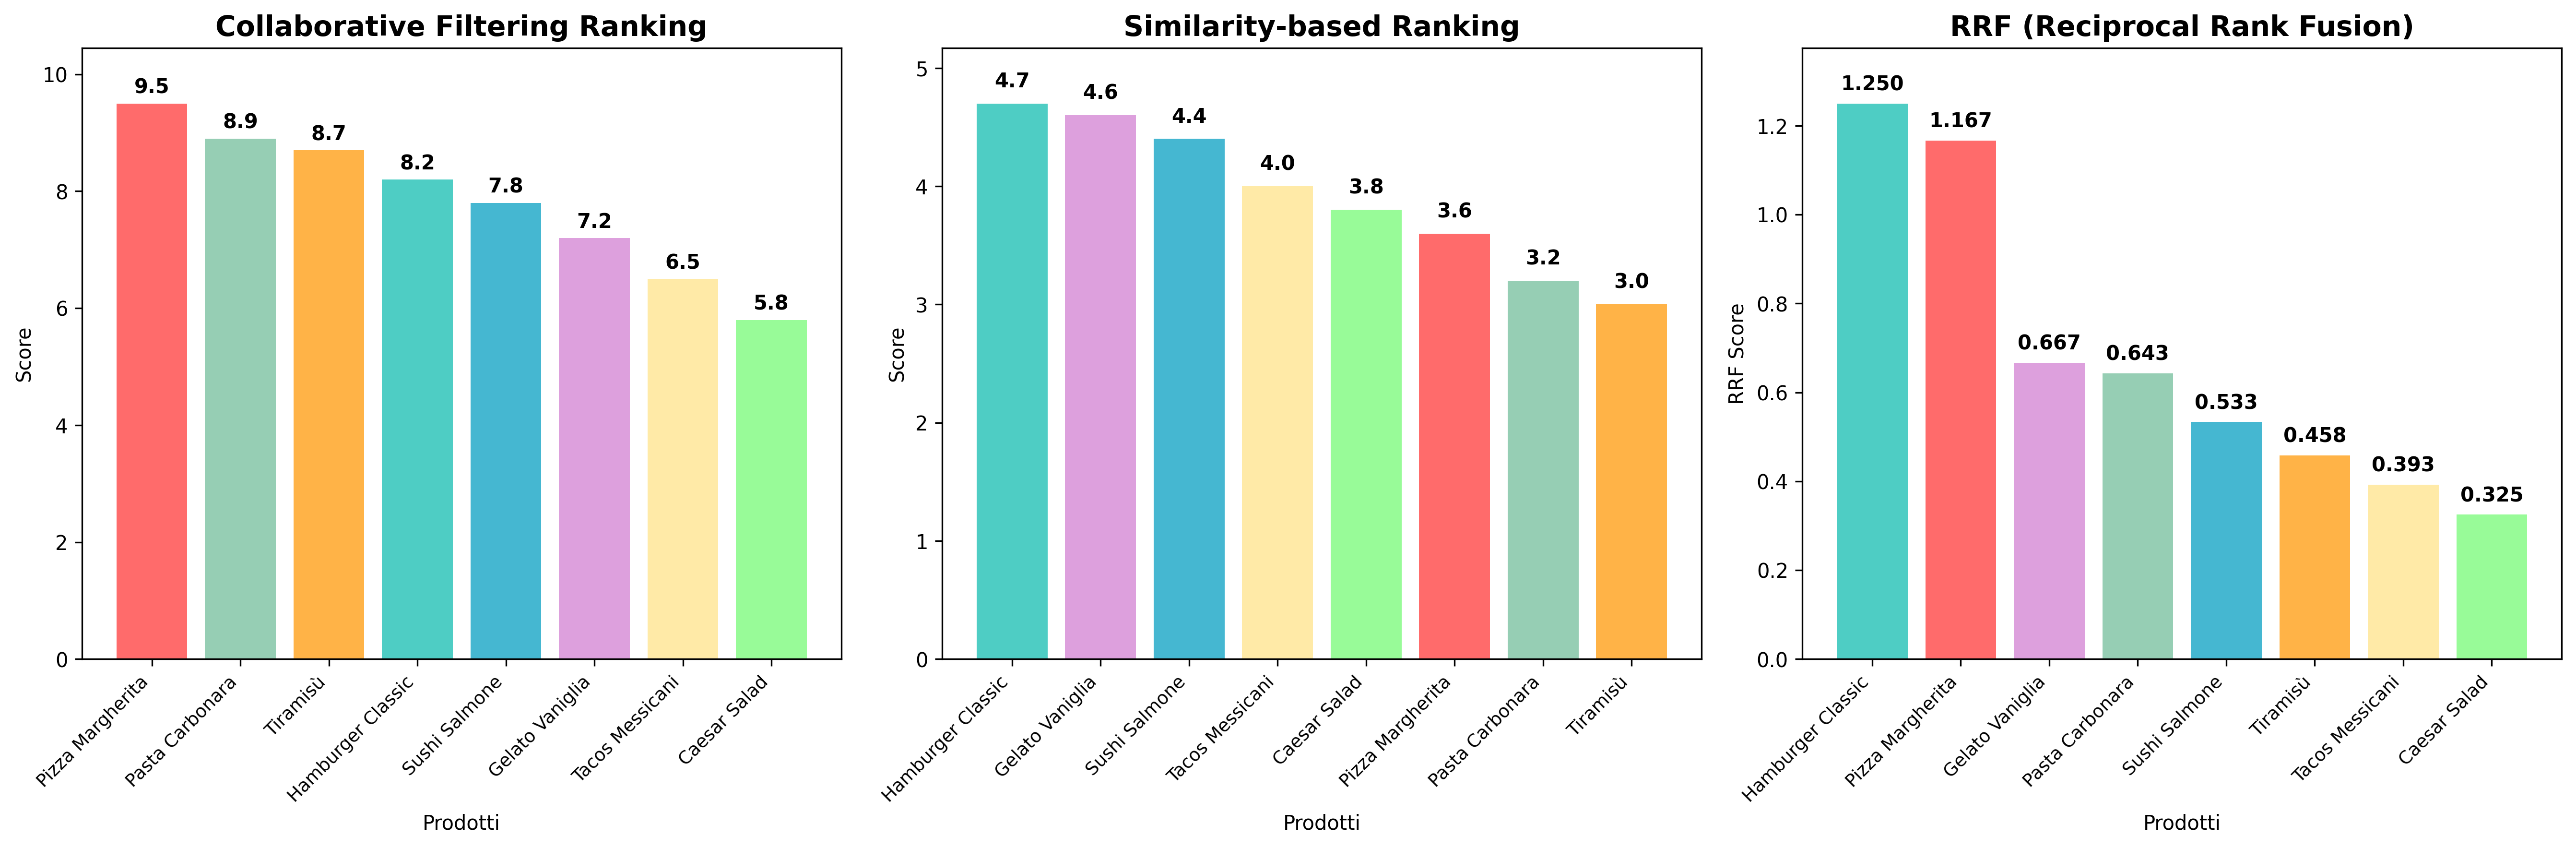
\includegraphics[width=0.8\textwidth]{rrf comparison charts/rrf_comparison_charts_toy_case.png}
    \caption{Esempio di Rank Fusion con RRF}
    \label{fig:rank-fusion-toy-case}
\end{figure}

Si può notare come tutti e 8 i prodotti siano rappresentati in tutti i rankings con lo stesso colore, per indicare che sono gli stessi prodotti, ma con posizioni diverse.
Il terzo ranking è il risultato della fusione dei primi due rankings, e mostra come i prodotti siano stati riorganizzati in base al loro punteggio RRF.

In particolare, considerando il prodotto "Hamburger Classic", il calcolo che viene fatto per il suo punteggio RRF è il seguente:

\begin{equation}
\text{RRF}(p) = \frac{1}{\text{rank}_{CF}(p)} + \frac{1}{\text{rank}_{Sim}(p)} = \frac{1}{4} + \frac{1}{1} = 1.25
\end{equation}

Oppure, considerando il prodotto "Pasta Carbonara", il calcolo che viene fatto per il suo punteggio RRF è il seguente:

\begin{equation}
\text{RRF}(p) = \frac{1}{\text{rank}_{CF}(p)} + \frac{1}{\text{rank}_{Sim}(p)} = \frac{1}{2} + \frac{1}{7} \approx 0.643
\end{equation}

E così via per gli altri prodotti. Si può notare come, nonostante i due rankings di partenza abbiano scale di punteggio diverse ("da 1 a 10" e "da 1 a 5"), il metodo RRF riesce a combinarli in modo efficace, poichè restituisce un ranking finale che tiene conto solo delle loro posizioni relative.

Al termine del processo di Rank Fusion, il sistema di raccomandazione restituisce un ranking finale dei prodotti, ordinato in base ai punteggi RRF calcolati. Questo ranking rappresenta dunque le raccomandazioni finali del sistema, che possono essere presentate agli utenti come suggerimenti personalizzati.

Un esempio di caso reale tratto dal dataset \texttt{Orders\_export.csv} è mostrato nella seguente immagine \ref{fig:rank-fusion-real-case}, che mostra i primi 10 prodotti raccomandati per il cliente \texttt{Ds-trading srl Ds-trading GmbH}.

\begin{figure}[h]
    \centering
    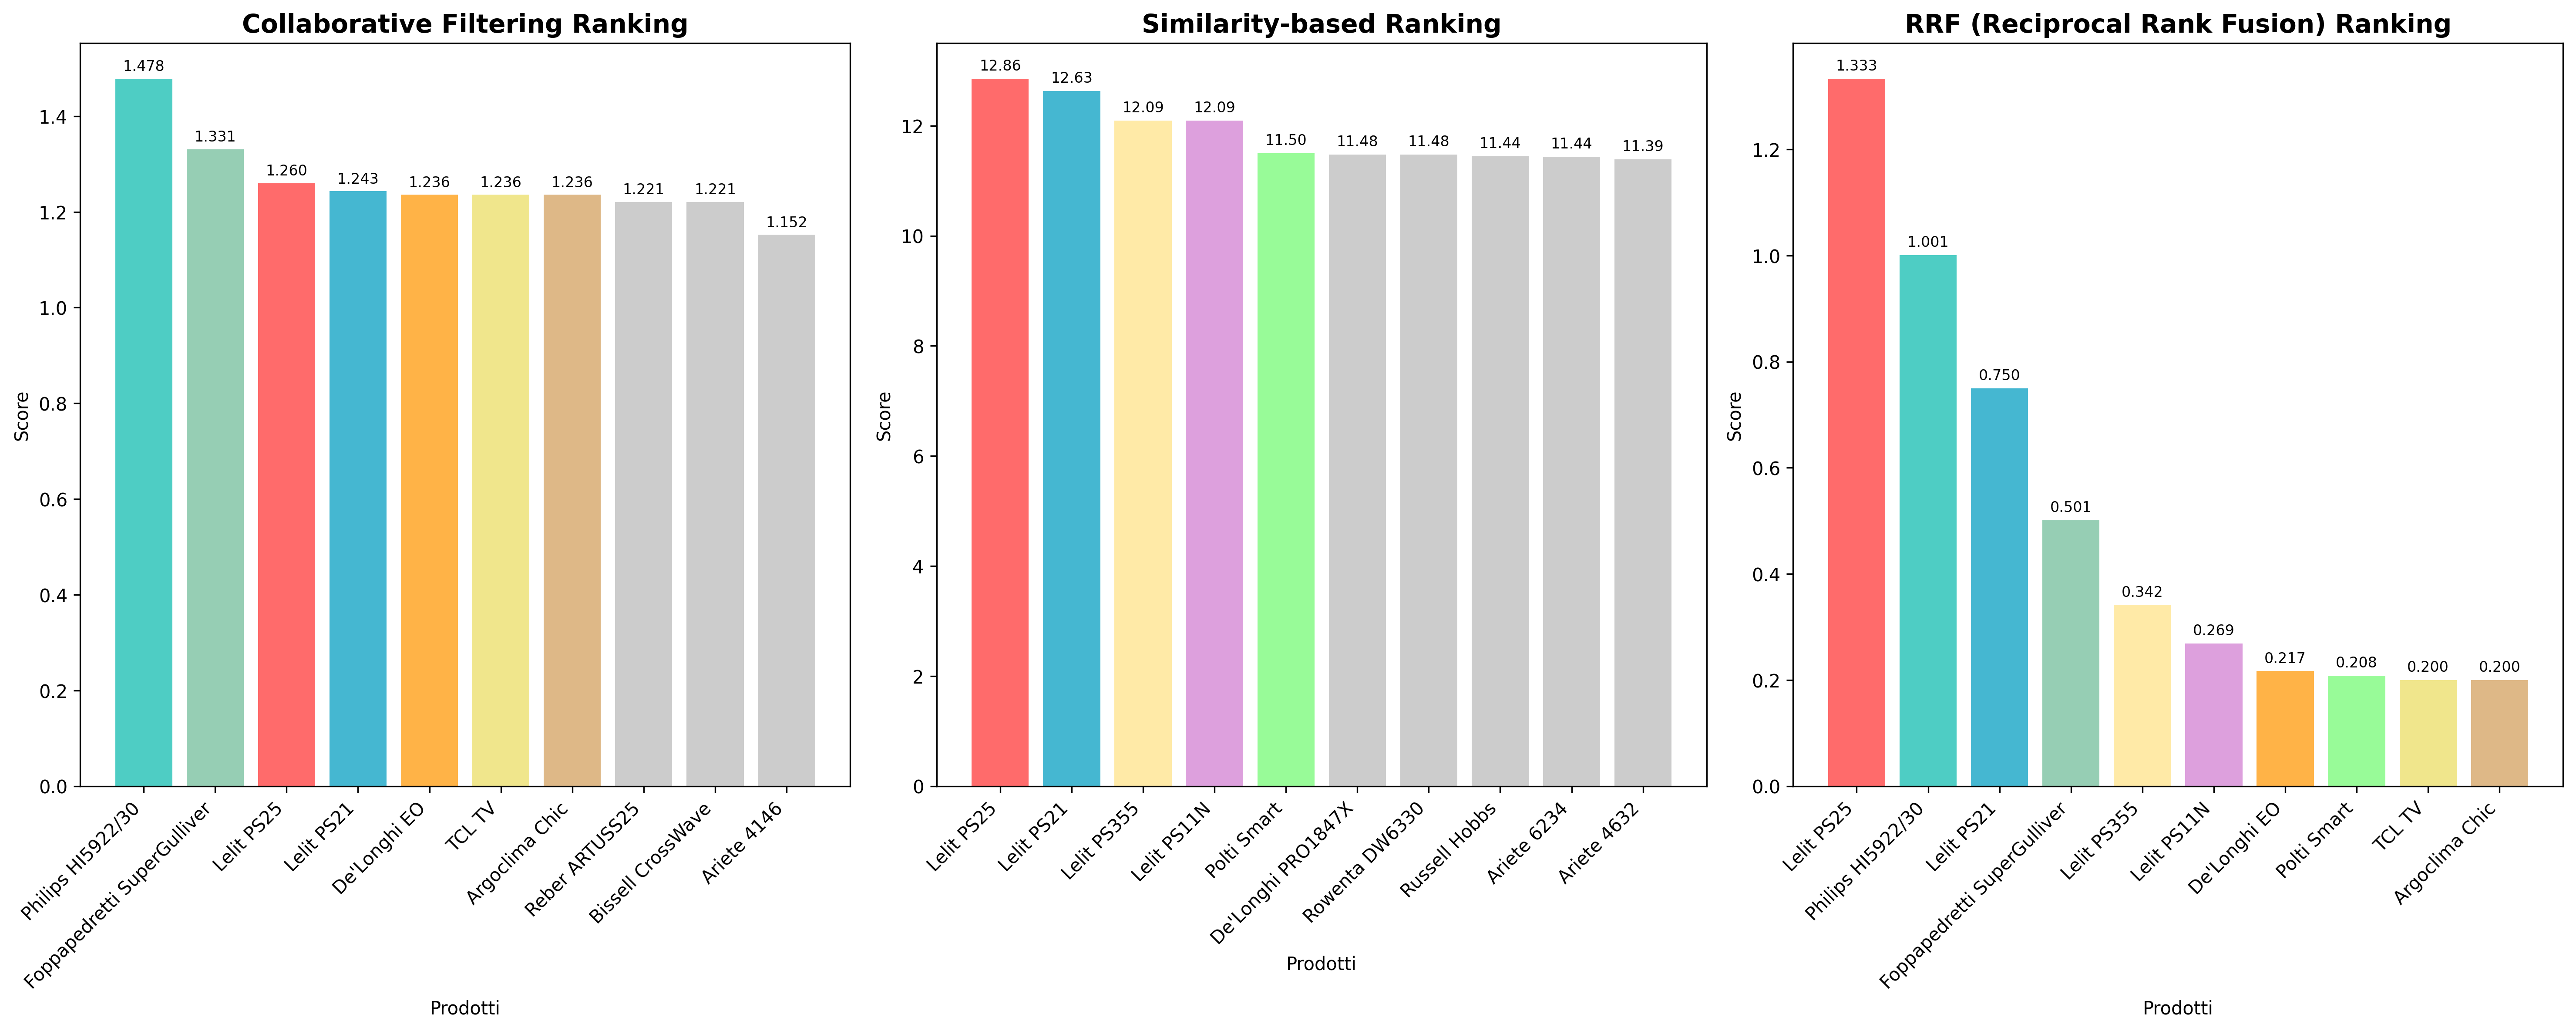
\includegraphics[width=0.8\textwidth]{rrf comparison charts/rrf_comparison_charts_real_case.png}
    \caption{Esempio di Rank Fusion con RRF su un caso reale}
    \label{fig:rank-fusion-real-case}
\end{figure}

Qui, si può notare come siano stati colorati tutti i prodotti presenti nel ranking RRF, ma, a differenza del caso giocattolo, questi prodotti non sono tutti visualizzati contemporaneamente in entrambi i due rankings di partenza, poichè il dataset contiene molto più di 10 prodotti, che è il limite di rappresentazione dei rankings in questi grafici, e quindi alcuni sono stati classificati più indietro. Inoltre, in questi due rankings originali sono visualizzati dei prodotti che non sono poi visualizzati nel ranking RRF finale, ed allora sono rimasti di colore grigio, per indicare che non sono stati raccomandati al cliente.

Il numero di raccomandazioni che il sistema restituisce viene configurato tramite apposito input dell'utente. In entrambi gli esempi mostrati, il numero di raccomandazioni è stato impostato a 10, ma questo appunto può essere modificato a piacimento.


\section{Filtro}

\section{Recbole e Surprise}

\section{Metriche}

\section{Serendipità}

\section{Explainability}
